
% JuliaCon proceedings template
\documentclass{juliacon}
\setcounter{page}{1}

\begin{document}

%% **************GENERATED FILE, DO NOT EDIT**************

\title{A Data Persistence Architecture for the SimJulia Framework}

\author[1]{Van Der Paelt Piet}
\author[1]{Lauwens Ben}
\author[2]{Signer Beat}
\affil[1]{Royal Military Academy, Renaissancelaan 30, Brussels, Belgium}
\affil[2]{WISE Lab, Vrije Universiteit Brussel, Pleinlaan 2, Brussels, Belgium}

\keywords{\mbox{Discrete-Event Simulation}, \mbox{Frameworks}, \mbox{Tools}, \mbox{Data Storage}, \mbox{Persistence}, \mbox{Julia}, \mbox{ConcurrentSim}, \mbox{ResumableFunctions}, \mbox{PostgresORM}, \mbox{Object-Relational Mapping}, \mbox{Metaprogramming}, \mbox{Macro Expansion}}

\hypersetup{
pdftitle = {A Data Persistence Architecture for the SimJulia Framework},
pdfsubject = {JuliaCon 2022 Proceedings},
pdfauthor = {Van Der Paelt Piet, Lauwens Ben, Signer Beat},
pdfkeywords = {\mbox{Discrete-Event Simulation}, \mbox{Frameworks}, \mbox{Tools}, \mbox{Data Storage}, \mbox{Persistence}, \mbox{Julia}, \mbox{ConcurrentSim}, \mbox{ResumableFunctions}, \mbox{PostgresORM}, \mbox{Object-Relational Mapping}, \mbox{Metaprogramming}, \mbox{Macro Expansion}},
}


%

\title{ A Data Persistence Architecture for the SimJulia Framework}

\author[1]{Van Der Paelt Piet}
\author[1]{Lauwens Ben}
\author[2]{Signer Beat}
\affil[1]{Royal Military Academy, Renaissancelaan 30, Brussels, Belgium}
\affil[2]{Vrije Universiteit Brussel, Pleinlaan 2, Brussels, Belgium}

\keywords{Discrete-Event Simulation, Frameworks, Tools, Data Storage, Persistence, Julia, SimJulia, ResumableFunctions, PostgresORM, Object-Relational Mapping, Metaprogramming, Macro Expansion}

\maketitle

\begin{abstract}
We present a novel transparent data persistence architecture as an extension of the SimJulia package. We integrated PostgresORM into the ResumableFunctions library by using Julia's metaprogramming support. As such, we were able to remove the dependency on a user's knowledge on architectures for persistence. Furthermore, we implemented two distinct approaches to externalise the data. The first one integrates our dynamic object-relational mapping (ORM) in the existing VueJS.jl package and a second one oriented towards a REST API, consumed by existing frameworks and application templates. Our contribution aims to improve the usability, whilst demonstrating the power of macro expansion to move towards a dynamic ORM configuration.
\end{abstract}

\section{Introduction}

The rationale behind simulation is to collect data on systems or processes that are more likely to be described by a model which can be evaluated numerically, rather than being subjected  to exact mathematical methods which produce an analytic solution\cite{law2007simulation}. Therefore, the goal is to generate data by means of simulation which in turn, allows for conclusions to be drawn on the system from which the model originated.\vskip 6pt

We focus on the SimJulia \cite{lauwens2017simjulia,lauwens2017simjuliaSite} Discrete Event Simulation (DES) framework implemented in the Julia Programming Language \cite{bezanson2017julia}. This framework is highly inspired by SimPy \cite{SimPy} and DISCO \cite{helsgaun1980disco}, which is a SIMULA \cite{DahlNygaard1966simula} class for combined continuous and discrete simulation. The framework has been adopted in diverse research projects situated in several domains, including the Medical \textit{(SIMEDIS: a Discrete-Event Simulation Model for Testing Responses to Mass Casualty Incidents} \cite{de2018simedis}), Human Resources \textit{(Manpower planning using simulation and heuristic optimization \cite{abdessameud2019manpower})} and Ballistics \textit{(Simulating a Stochastic Differential Equation Model by Exact Sampling \cite{hermosilla2017ballistics})}\vskip 6pt

Abar et al. \cite{abar2017agent} consider an extensive list of Agent-Based Modelling and Timulation (ABMS) tools, both open source and proprietary. A categorisation, amongst others, on the model development effort is made. furthermore, Abar states \textit{"An ideal simulation system should require minimal learning effort as well as provide flexible support to creating models and running robustly on any type of computing machine."} We share that thought. Moreover, since SimJulia is a process oriented framework, in which a simulated entity can be seen as an independently coded agent, SimJulia merits its place amongst other ABMS tools as considered by Abar. \vskip 6pt

We feel Abar's statement can be extended to the monitoring and persistence aspect. To the best of our knowledge, none of the open-source frameworks provide an easy-to-implement data storage mechanism. It is our observation that monitoring creates an additional burden for an end-user due to the dependency on knowledge of technology for persistence and how to interact with it from within the simulation model, regardless of the chosen programming language or implementation. Our goal is to lower that burden by removing this dependency. \vskip 6pt

Currently, SimJulia lacks the functionality to transparently store state variables which characterise the evolution of a running DES model as well. To mitigate this shortcoming, we extended both the SimJulia and the ResumableFunctions \cite{lauwens2017resumablefunctions} packages by implementing a transparent probing and data persistence architecture, employing Julia's metaprogramming support. Our implementation uses the Object Relational Mapping (ORM) concept \cite{russell2008bridging} implemented in the PostgresORM package \cite{tecnivelPostgresORM}, supported by the PostgreSQL Relational Database Management Systems (RDBMS) \cite{psqldocs}. The high level architecture of our implementation is depicted in figure \ref{fig:highlevelarch}.

\begin{figure}[th]
	\centering
	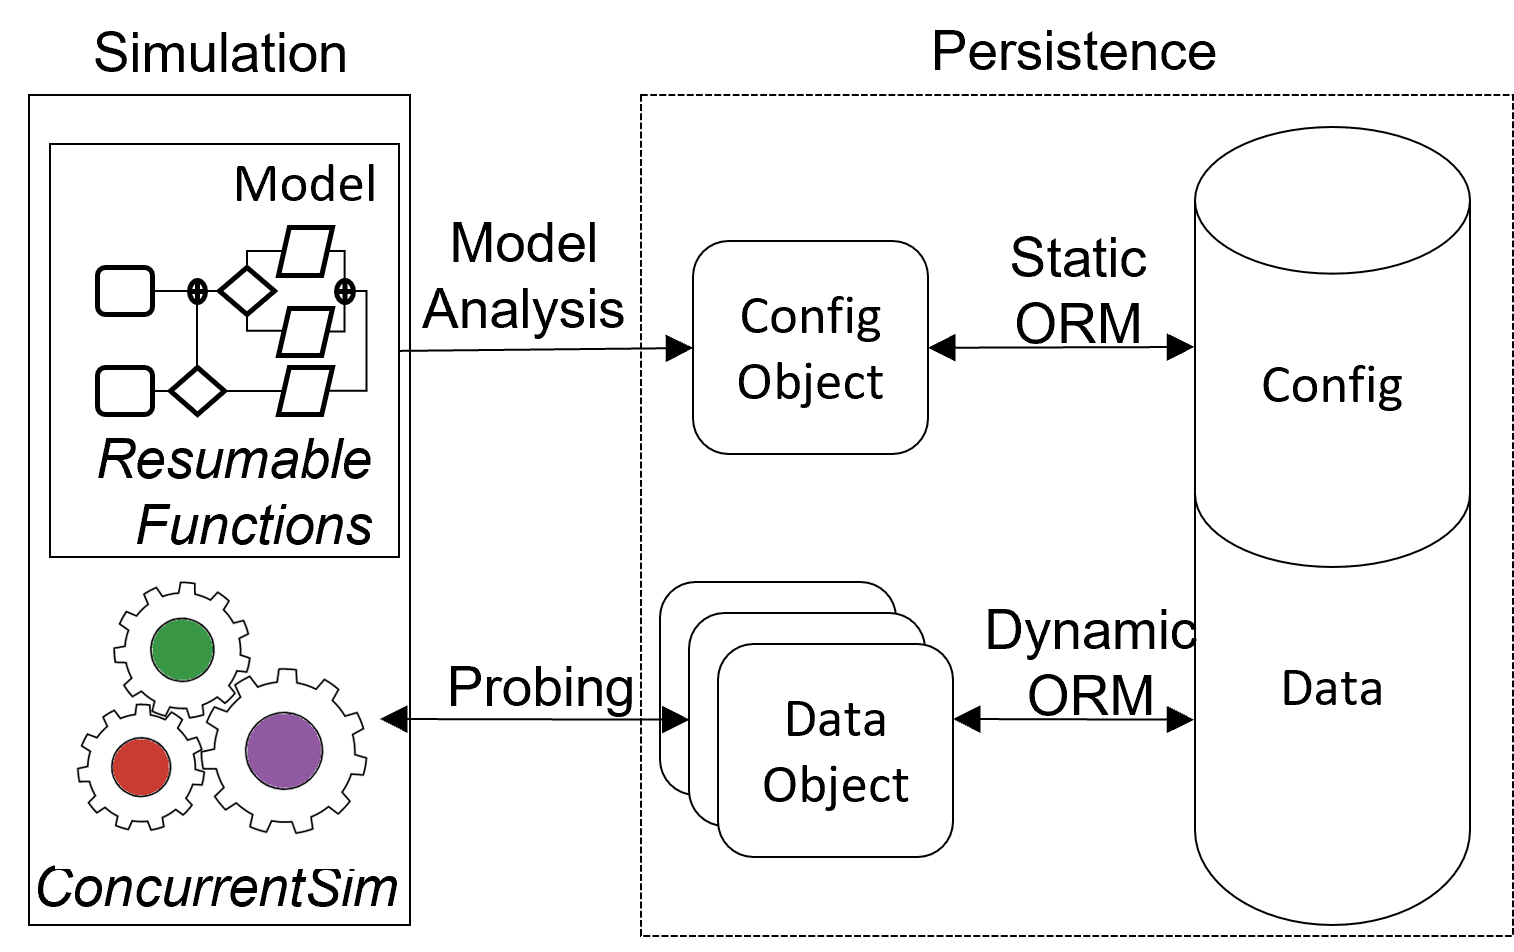
\includegraphics[width=0.9\linewidth]{images/HighLevelArch}
	\caption{Persistence: High Level Architecture}
	\label{fig:highlevelarch}
\end{figure}

High level, we distinguish a static phase, during which model analysis takes place, from a dynamic phase, during which a simulated system is probed to retrieve generated data. Both phases use an ORM to store data, respectively using a static setup and a dynamic setup.\vskip 6pt

The remainder of our text is structured as follows: in section \ref{MainPackages} we present the Julia Packages we used to implement our architecture. We continue by a detailed description of the implementation in section \ref{PArch}.\vskip 6pt

\section{Related Work}\label{MainPackages}

In this section we present the main Julia packages which relate heavily to our architecture. It mainly concerns the ResumableFunctions.jl, ConcurrentSim.jl and PostgresORM.jl packages.\vskip 6pt

\subsection{ResumableFunctions.jl}
ResumableFunctions.jl \cite{lauwens2017resumablefunctions} implements the macro's \texttt{@resumable} and \texttt{@yield} which transform plain Julia functions in functions which can be interrupted during evaluation with the possibility to be resumed afterwards.\vskip 6pt

The argument of the \texttt{@resumable} macro is a function definition, which, in the context of this work, represents a process we want to simulate. Several internal functions rewrite the argument-function's body. The resumable character is essentially realised through the substitution of the \texttt{@yield} macro by a return statement, followed by a label to which the iterator can jump to upon resuming execution. This new body constitutes the definition of a finite-state machine. Using MacroTools.jl \cite{macrotools}, it is integrated in a function which, when called, results in the Finite Sate Machine Interface (FSMI). That FSMI is subsequently assigned to a field in a callable mutable struct which also contains the variables included in the FSMI, and a field which holds the current state of that FSMI. Lastly, a function definition is generated which bears the same signature as the original argument-function. \vskip 6pt

A first call to that new function leads to the initialisation of the callable mutable struct, including the creation of the FSMI instance. The return of this function call is the instantiated callable struct. Subsequent calls to this returned callable struct step through the finite state machine, causing state variable to get updated. Finally the end-state is reached. \vskip 6pt

\subsection{ConcurrentSim.jl}

Previously known as SimJulia.jl, ConcurrentSim.jl \cite{lauwens2017simjulia,lauwens2017simjuliaSite} is the event-driven simulation framework which we extended with automated persistence features. \vskip 6pt

A simulated system consists of processes which are defined as (nested) resumable functions, and a simulation environment. The latter holds the datastructures containing necessary to run the simulation. The simulation environment is a mandatory argument to each of the resumable functions. \vskip 6pt

The top-level process is initialised through an instantiation of it's corresponding callable mutable struct as an argument to the \texttt{@process} macro in the global scope. Other processes can be nested in functions as well by means of the \texttt{@process} macro in a local function scope. Having defined the simulation model and the environment, the simulation can be run through a call to the \texttt{run} function. The latter takes the simulation environment as an argument. \vskip 6pt

Upon evaluation of the top-level process, the \texttt{@process} macro causes an event to get scheduled on the heap of the simulation environment. This heap is in fact a priorityqueue provided by the package DataStructures.jl \cite{datastructures}. The event has an array of callback functions which gets appended functions that need to be executed once the event occurs. \vskip 6pt

Finally, the \texttt{run} function runs the simulation in a stepped way. The first event in the priority queue is dequeued and its corresponding array of callback functions gets executed. All Events that are scheduled on the simulation heap occur in this way. Nested functions cause events to get scheduled as well, albeit with a different priority. This approach allows for chaining of events which cycle through the states of the different processes such that the execution of the simulation corresponds to the model which defined it. \vskip 6pt

\subsection{PostgresORM.jl}

PosrgresORM.jl \cite{tecnivelPostgresORM} provides Object Relational Mapping (ORM) \cite{russell2008bridging} between a Julia project and a PostgresORM database. Data lives in an application and needs to travel back and forth between the database and the application itself. Standard SQL could provide a bidirectional interface between both, but this comes with the downside a programmer needs to master the technology. PostgresORM.jl provides a bidirectional interface, and is based on three separate, straightforward to configure, internal modules. \vskip 6pt

The package provides several functions which map directly to Create, Read, Update and Delete (CRUD) operations. All of these functions take an object as an argument. Depending the nature of the function it was passed to, the object is persisted or used as a filter object in the context of an SQL where-clause. The object possesses uniquely identifying attributes, which translate into primary key attributes in the relation. \vskip 6pt

\section{Persistence Architecture}\label{PArch}
The architecture's main design principle is to probe a running simulation model for its current state variable values, and store this information in a persistent way for later exploitation. The array of callback functions gets executed after the occurrence of each event, and is therefore suitable for invoking the probing function.
This concept is illustrated in figure \ref{fig:cbprobing}. After an event "Event1" got executed, the array of $n$ callback functions $c_i$ gets executed, where $c_n$ is the probing function itself.

\begin{figure}[th]
	\centering
	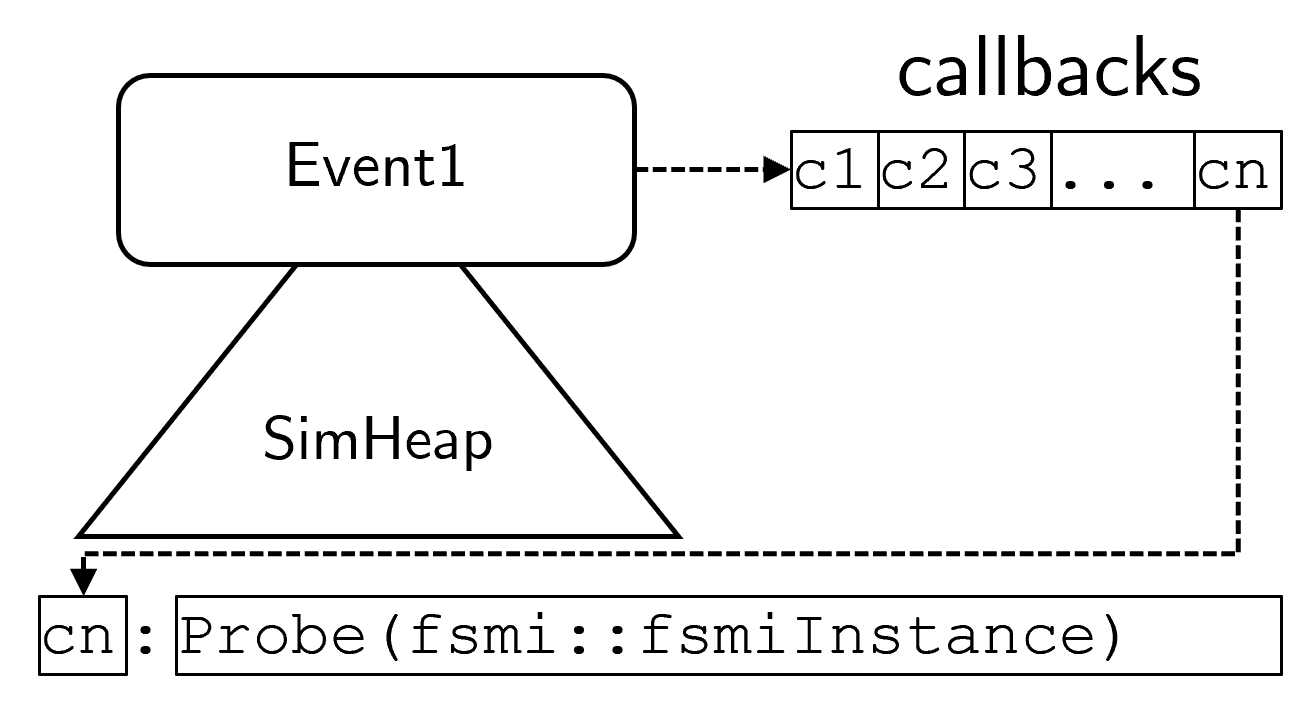
\includegraphics[width=0.9\linewidth]{images/simHeapCallbacksProbe}
	\caption{Event Callback Functions: Probing}
	\label{fig:cbprobing}
\end{figure}
 However, since active processes switch back and forth, the probe might collect a different set of variables after the occurrence of each event. For this reason the probe needs to be aware of the kind of the active process. The latter implies the need to pass the FSMI itself as an argument to the probing function. In its turn, this results in the correct set of state variables. This set gives rise to an object which includes the necessary fields for every process, which must be persisted to the database. \vskip 6pt

This is closely related to the definition of an ORM, which is the technique of choice to persist data. Often, ORM's have a static configuration to determine which objects can exist and to which relations and attributes they map. PostgresORM \cite{tecnivelPostgresORM} uses the same approach, using modules to achieve this. Macro expansion allows to generate these modules dynamically at compile time. This strategy is fully exploited in our implementation. The concerned macro's take as an input the configuration for an ORM and produce the PostgresORM compatible modules. As such, a dynamic ORM is realised. The probing function selects a suitable object instantiator function and persists the object in the correct relation due to the mapping module. Multiple simulation runs can benefit the same macro expansion.\vskip 6pt

To retrieve the necessary input which drives these macro's, we must analyse the model under consideration. It is however unnecessary to execute this analysis prior to each simulation run. If the simulation model remains unchanged, the data model, hence the state variables that need to be persisted remain stable as well.\vskip 6pt

ResumableFunctions.jl performs such an analysis at compile time due to the macro \texttt{@resumable}. Our architecture benefits from this implementation to retrieve and store the simulation model's metadata. This model metadata is stable and needs to remain available throughout several simulation runs and must therefore be persisted separately. Therefore, a classic usage of a static ORM is suitable in this case.\vskip 6pt

The inner workings of our novel architecture described so far lead to an implementation in three phases, which require a different infrastructure to be provisioned:

\begin{enumerate}
	\item In a first phase, the simulation model is analysed. Static programming logic and infrastructure is used to retrieve and hold model metadata for internal exploitation.
	\item In a second phase, the dynamic ORM is realised through macro expansion, driven by the metadata gathered in the first phase. To persist data, dynamic infrastructure, dependent on the model under consideration is created and used to persist data.
	\item In a third phase data is visualised using the data model which was created in the previous phase. Additional frameworks and approaches such as a REST-api and a vue.js data interface are provided.
\end{enumerate}

In the remainder of this section, we will explain how these three phases are implemented in terms of programming logic and database configuration.

\subsection{Static Architecture}\label{statArch}

The starting point for each simulation is the definition of the model as resumable functions. We benefit from this macro expansion step to store the extracted information about the state variables (slots), present in the function. For this purpose, we extended ResumableFunctions.jl in two ways: (1) the macro now additionally saves metadata about the model itself and the slots present in each process and (2) takes a second boolean argument either to persist or not the evolution on the state variables. The latter merely adds the process's friendly name to a globally defined array which is used to communicate to the probe. That way the function "announces" itself as a monitored function.\vskip 6pt

The \texttt{@resumable} macro internally depends on the existing \texttt{get\_slots} function. Here, we introduced our new \texttt{saveSlotsToDb(origFuncName,slots)} function which (1) saves information about the version of the model through the function \texttt{createVersionRecord}, (2) saves the configuration of these slots to the database through the \texttt{createDataConfigRecords} function and (3) creates the relations that will hold the data for the function/process under consideration through the \texttt{dataTableBuilder} function. \vskip 6pt

The function \texttt{createVersionRecord} creates a \textit{modelmetadata} record in a dedicated relation if the model did not exist before. In the other case the concerned record gets updated. The primary key for such a process is the function name (that was originally passed to the @resumable macro), along with a hash of the slots. The relation holding information about the process under consideration includes the attributes name, hash of the slots, UUID, model creation timestamp and last used timestamp. To store the data, a static ORM was defined which is used to query the relation for the primary key of the process under consideration. Should the key exist, then the last used timestamp gets updated. In the other case, a record gets created. \vskip 6pt

After having saved the metadata concerning the current process, metadata concerning the process's specific slots is saved through the \texttt{createDataConfigRecords} function. This function provides the necessary information to the macro's that create the dynamic ORM. In the dedicated \textit{objectclassdefinition} relation, each slot's metadata is stored to feed these macro's: object and relation name, the object's field name, the data type, the mapping attribute and information whether the field participates in a primary key or not. This is realised through two static ORM definitions which point to the same relation. \vskip 6pt

Both of the relations we considered so far are statically defined. The attributes are known upfront, which allowed for a static ORM and an unvarying SQL DDL statement. The relation necessary to persist the slots of a process during the simulation is different since the attributes may vary depending on the slots present in the process. Therefore a dynamic SQL DDL statement needs to be established and executed for each new process. This is the task of the \texttt{dataTableBuilder} function which builds and executes the SQL DDL for each process. We benefit the SQL "IF NOT EXISTS" constraint to skip the creation for tables that already existed due to prior simulations of a certain process, including a same set of slots. \vskip 6pt

The architecture requires a PostgreSQL database instance running with a dedicated schema present. The schema must contain both of the statically defined relations: modelmetadata and objectclassdefinition. Access must be granted to a specific user for connections from static and dynamic ORM definitions. The schema holds the dynamically defined relations as well. \vskip 6pt

\subsection{Dynamic Architecture}

Given the availability of model and processes metadata, probing and persistence of a running simulation model is possible by using that metadata in the dynamic part of our architecture. The starting point is the newly added \texttt{@runPersisted} macro to ConcurrentSim, which must be used to start a simulation  instead of the \texttt{run} function, which remains available as well. The newly added macro performs two functions: (1) it includes the \texttt{ProbeApp} module which is a dynamically created module, dependent on the gathered metadata and (2) designates which dynamic-ORM provided object instantiator functions are used to probe which processes. \vskip 6pt

\subsubsection{The \textnormal{\texttt{ProbeApp}} Module}\hfill\\

\texttt{ProbeApp} is the module which implements the internal \texttt{Model} and \texttt{ORM} modules that make up a standard PostgresORM configuration. Both of them are implemented as macro calls: \texttt{@makeObjectDefModule} and \texttt{@makeOrmDefModule} respectively for Model and ORM creation. These macro's share the design principle that they both exploit metadata collected in the static part of the architecture described in the previous section \ref{statArch} , which alters the standard static approach of PostgresORM to the novel dynamic behaviour.\vskip 6pt

\paragraph{\textnormal{\texttt{@makeObjectDefModule}}}\hfill\\

The aim of \texttt{@makeObjectDefModule} is to build a PostgresORM-compliant module containing object definitions synthesised from the records available in the objectclassdefinition table. The task is accomplished by building an expression which evaluates to the \texttt{Model} module which configures PostgresORM. The object definitions included in this expression are created through mapping the \texttt{objToObjDef} over an array of metadata objects which originated from the table. Only the attributes of interest are retained in the record to metadata-object translation. The same static ORM we used previously to store data in the concerned table is now used to query it. A secondary task of the macro is to identify the current model's instantiator functions, since the probe will use only these later on. These are added to an array which becomes available in the global scope after evaluation of the macro. \vskip 6pt

\texttt{objToObjDef} realises individual struct definitions. It does so for what is concerned the fields of the struct by means of string interpolation in a quoted expression. Further, the function also uses MacroTools.jl's \texttt{combinedef} to generate both of the necessary positional and keyword constructor functions to comply with PostgresORM's requirements. As such, \texttt{objToObjDef} is an aggregating function on the metadata objects.\vskip 6pt

\paragraph{\textnormal{\texttt{@makeOrmDefModule}}}\hfill\\

The inner workings of \texttt{@makeOrmDefModule} are very similar to \texttt{@makeObjectDefModule}. The macro evaluates to an \texttt{ORM} module which is internal to PostgresORM and works in tandem with the object definition created through the evaluation of the \texttt{@makeObjectDefModule} discussed earlier. Each object definition requires the corresponding ORM.\vskip 6pt

Metadata objects resulting from the objectclassdefinition table serve as an input to the function \texttt{createOrmsFromDB}, which generates the ORM modules dynamically on a per-object basis. The final module body is generated through string interpolation in a quoted expression.\vskip 6pt

\subsubsection{The \textnormal{\texttt{SimProbe}} Module}\hfill\\
Probing and persistence is realised through the module \texttt{SimProbe}, which exports the probing function, and acts upon the different (sub)processes. The probing function is activated through inclusion in the array of callback functions which get executed when an event occurs. \vskip 6pt

\paragraph{Probe Implementation}\hfill\\

The module \texttt{SimProbe} implements the probing function \texttt{ProbeStructured} which takes the FSMI instance as an argument. To comply with ConcurrentSim.jl a wrapper function \texttt{Probe} exists as well. A mapping dictionary available at the main simulation environment struct provides the information if the FSMI instance under consideration is truly a monitored process through the presence of the corresponding object instantiator function. The probing function transfers the variables present in the FSMI to a corresponding struct. The latter is then persisted to the database. This mechanism relies entirely on the availability of the dynamic ORM which lives in the global scope through macro expansion from within the module \texttt{ProbeApp}, and on the coupling of FSMI types to the correct instantiators.\vskip 6pt

\paragraph{Probe Activation}\hfill\\
The \texttt{probe} function is activated using the array of callback functions. The evolution of the variables in a running simulation maps to the evolution of the state variables in the corresponding state machine. The latter is representation of a (sub)process contained in the simulation model. To capture state variables, the full array of callback functions must be executed first. Only then, a state machine can make a transition from one state to another, or in other words, proceed to the next event. We added the \texttt{probe} function as a callback function.\vskip 6pt

The last shackle that joins together the the two chains of necessary infrastructures is the coupling of the type of the FSMI to the correct instantiator. This is only possible when the static phase has terminated, and the dynamic phase is beyond the evaluation of the \texttt{SimProbe} module. At this moment, we dispose of the information which functions must be monitored, and how their ORM's should look like. Furthermore, through the dynamic phase, the necessary ORM's are in place. At this stage, the ORM's are availabe to the \texttt{SimProbe} module to create and store shadow objects for each monitored process. The coupling of the type of the FSMI to the instantiator is executed just before the simulation starts. The newly added macro \texttt{@runPersisted} performs this function. It iterates over the globally defined array of processes that need to be monitored (those who "announced" themselves) and designates instantiator functions to FSMI types. This information is stored at the top-level simulation environment struct which was extended for this purpose.\vskip 6pt

\subsection{Data Visualisation}
To visualise the data gathered using the techniques described earlier, we devised two distinct approaches which share the same goal: a user should have access to all persisted data in tabular format from within a web browser. The first approach is an integrated solution which includes a web application running in a single thread, mainly based on the VueJS.jl package. The second approach consists of a REST architecture combined with an existing web framework.\vskip 6pt

\subsubsection{Integrated Web Application}\hfill\\

We used VueJS.jl as proposed in the technical documentation. A router is defined in a global scope, on which several routes are registered. Such a route consists of a combination of a virtual directory and one of the http request modes. When requested, a route invokes a function which returns a well-formatted html page which gets served upon the request arriving from a http client.\vskip 6pt

The VueJS.jl package intervenes in the local scope of such a function, exposing several html elements enriched by the original Vue.js framework. Apart of some static definitions, our application is centred around two functions. \texttt{showDataTables} implements the landing page and shows a list of processes which corresponds to all processes ever persisted in the connected schema. Upon selection of a process, a parametrised http GET request is made against the http server invoking the \texttt{showTable} function. The latter builds the page containing the appropriate data table. \vskip 6pt

Our contribution is situated at the level of these two functions. They integrate our earlier, both statically and dynamically, defined ORM's. Whereas these ORM's had a role towards data persistence earlier, they are  now employed in data retrieval. To do so, the \texttt{ProbeApp} module is imported in the application's global scope. \texttt{showDataTables} uses the static ORM to retrieve the list of processes available in the schema. To do so, an unconfigured filter object is sent to the schema. The result is used to populate the list of possible processes at the landing page. Selection of one of these processes invokes the \texttt{showTable} function which is aware of what kind of filter object to send to the schema.\vskip 6pt

Since VueJS.jl is highly oriented towards dataframes, as implemented by DataFrames.jl, and the ORM's return a resultset comprised of objects, a utility function bridges the gap between the two. It allows to send any filter object to a schema, and receive the appropriate dataframe in return.\vskip 6pt

\subsubsection{REST Oriented Architecture}\hfill\\

The REST oriented architecture consists of a Julia implementation of the REST api combined with an application running in the node.js ecosystem. We implemented the application using the vue-crud \cite{masny2018vuecrud} framework. We also implemented a second application directly using vue components.\vskip 6pt

\paragraph{Rest API}\hfill\\

The server side of the REST application is implemented using the HTTP.jl package. A http server listens at a given port for a request for a virtual directory. The required table, which maps to a monitored process, is now passed to the server as a virtual directory in the requested URL, and gets extracted using the positional pattern matching features provided by the HTTP.jl package. Together with the HTTP method ("GET"), the server is aware the request is a READ operation on a certain table.\vskip 6pt

The base implementation is highly inspired by the Cross-Origin Resource Sharing (CORS) example from the HTTP.jl documentation \cite{httpjl}. However, in our implementation, a request arriving at the server invokes a service function \texttt{getTableContent} which will request the data from the back-end database. Since the \texttt{ProbeApp} module is imported in the global scope where the HTTP server runs, and the required table was passed as a positional parameter (virtual directory) in the URL, we are able to instantiate the correct filter object for the required table and pass it to the ORM's \texttt{retrieve\_entity} function. The resultset is then transformed to the correct JSON format using the \texttt{JSONMiddleware} and \texttt{CorsMiddleware} functions as provided by the http.jl documentation. These two functions implement the CORS-oriented aspects as well. For the inner workings of the two latter functions, we refer to the documentation.\vskip 6pt

\paragraph{Vue-CRUD Application}\hfill\\

Vue CRUD is a node.js framework which can be used to create, amongst others, Customer Relationship Management (CRM) applications which communicate with the server via a REST API. In our implementation, it is the framework of choice to consume the REST API due to its completeness and ease of deployment. Vue-CRUD is part of a larger, encompassing suite "What CRUD!" which also includes the Laravel-crud-api. The latter is the accompanying REST API implemented in PHP and Laravel. In our project, this component was replaced by the REST API implemented in Julia. Using this framework, we prove the required (offering an open-standard interface to the data) functionality was delivered. \vskip 6pt

To use the framework, a node.js server was installed and the framework was deployed as described in the documentation. Amongst the available templates, the "simple-crud" template was deployed and configured with the intention to visualise a single table residing in the schema.\vskip 6pt


\paragraph{Vue Application}\hfill\\

To facilitate a comparison of a Vue-CRUD configuration against a native Vue implementation, a dedicated Vue app was developed which offers the same functionality as the Vue-CRUD deployment. The prerequisites for such an app are very similar: a running node.js server is required with the Vue module available. At the centre of the implementation itself resides the Axios \cite{axios} library which is used to consume the REST API. The solicited endpoint is encoded by means of it's URL which is passed to the Axios \texttt{get} function, resulting in a data object which holds the retrieved JSON file. An iteration over this data object using Vue's \texttt{v-for} inline directive is used to generate the inner rows of a html table.\vskip 6pt

% **************GENERATED FILE, DO NOT EDIT**************

\bibliographystyle{juliacon}
\bibliography{ref.bib}


\end{document}

% Inspired by the International Journal of Computer Applications template
